
\section{Project Management}
\subsection{Agile}
First described in the Manifesto for Agile Software Development \cite{beck2001manifesto}, Agile development is a set of principles and methods for project management. The Agile methodology is characterized by an iterative, approach to software development \cite{cockburn2001agile}. There is a strong emphasis on embracing the change and uncertainty normally associated with software development projects. The goal is to continuously deliver working software while simultaneously refactoring and tweaking as the development process unfolds.  

\subsubsection{Kanban}
The Kanban method is highly visual and aims to illustrate each stage within a process and the interconnectedness between them \cite{sugimori1977toyota}. The basic structure of the Kanban system is a storyboard. The board is split into different lists that represent the consecutive stages of completing the work. Within each list are cards. These are the smallest work units, or simply put, a task. The Kanban process, in essence, is moving a card (a single task) from left to right on the board. On the left-most side is the To Do list – and the task is gradually pushed to completion until it reaches the Done list. Because the board offers a clear overview of all tasks and their progress, it’s easy to see where any work gets stalled

\subsubsection{SCRUM}
The SCRUM method is based on the work of Pittman and Booch \cite{pittman1993lessons}. The focus of Scrum is addressing software development in a flexible way through the use of \say{inspect and adapt feedback loops}. Time is divided into short work cadences, known as sprints, typically one week or two weeks long.  At the end of each sprint, stakeholders and team members meet to discuss the progress of the previous sprint and plan for the next sprint. 


\section{Tech Review}

The following section outlines the key tools and technologies used during the development of this project.


\subsection{Project Management Tools}

\subsubsection{Github}
Git is an open source distributed version control system that allows content to be tracked by maintaining a history of changes. GitHub is a code hosting platform that implements Git for version control and collaboration.
\subsubsection{Trello}
Trello is an online project management tool that facilitates the creation of storyboards. A storyboard can represent a stream of activity or an entire project. Boards, lists and tasks can be created via Trello's user interface. 


\subsection{Developer Tools}

\subsubsection{Atom Editor}
Atom is a free, open source text editor. It features support for Windows, Linux and macOS, and takes the form of a desktop application. Built using Electron, CoffeeScript and HTML, Atom’s key feature is its customizability. Developers are encouraged to write their own plugins and as a result, it has been dubbed the \say{Hackable editor of the 21st century}\cite{atom}.
Github is the chief contributor to the Atom project and as a result, Atom has Github integrated at its core. The GitHub package for Atom allows developers to create new branches, stage and commit, push and pull, resolve merge conflicts, view pull request - all from within the editor. 


\subsubsection{Nuclide}
Nuclide is a set of packages that adds IDE-like functionality to Atom. Developed by Facebook, Nuclide is built on top of Atom’s source code, providing pre-configured optimizations and customizations. Nuclide has strong support for web and mobile development. While Nuclide has been shown to consume more memory than Atom alone, it adds substantial functionality.\cite{nuclide} 

\subsubsection{Quick Open}
Quick Open is one of the most notable features of Nuclide. The Quick Open technology gives access to Nuclide’s file search mechanism, including OmniSearch, which quickly displays recently opened files, quick searches for files based on partial names, and depending on the project, can search within files for symbols\cite{quickopen}.


\subsubsection{Unity}
Unity is a cross-platform real-time engine developed by Unity Technologies. Unity allows developers to create games and interactive experiences in both 2D and 3D. The central scripting API is compatible with the C\# programming language. The Unity editor supports the creation of content for a wide variety of platforms ranging from gaming consoles to mobile devices on Android, iOS, and Windows \cite{unity}. 

\subsubsection{Android Studio}
Android Studio is the de-facto IDE for developing Android applications. Android Studio features gradle-based build support, refactoring tools, lint tools, a virtual android device emulator and built-in support for the Google Cloud Platform and Firebase. It also supports development in all languages of IntelliJ, for example, Java, Koltin and C++. Android studio is supported on Microsoft Windows, Mac Os and Linux distributions \cite{android_studio}. 


\subsection{Application Development Tools}

\subsubsection{Typescript}
TypeScript is a superset of JavaScript which provides functionality for static typing, classes and interfaces \cite{typescript}. The core purpose of Typescript is to enable IDEs to provide developers with a more complete development environment.  The IDE is informed in real-time by the TypeScript compiler on its rich type information. This allows the developer to catch bugs and errors early in development. Furthermore,  static typing helps establish a more robust codebase.

\subsubsection{Typescript Compiler}
 Typscript code is transcompiled into regular JavaScript and can then be executed in any JavaScript engine (e.g. a browser). As TypeScript is a superset of JavaScript, existing JavaScript programs are also valid TypeScript programs. 

\subsubsection{Node}
NPM(Node Package Manager) is a software package manager and installer. It is the world’s largest software registry and contains over 800,000 code packages \cite{npm}. While NPM is primarily used to share open source software, many organizations use it to manage private development. NPM packages are defined in JSON and stored in a  package.json file. The management of dependencies can also be handled by npm. Dependencies are defined and shared in the package.json file. 

To install NPM, Node.js must be present on the machine. Node.js is a free, open-source server environment. It supports a myriad of platforms including Windows, Linux, Unix, Mac OSX and more.  The name npm (Node Package Manager) stems from when npm first was created as a package manager for Node.js.


\subsubsection{Angular JS}
Angular JS is an open source JavaScript framework used for front-end development. Its goal is to help manage the complexity associated with client-side javascript code. Angular JS extends the traditional functionality of HTML through the use of additional attributes to make the code more responsive and expressive \cite{angularjs}. 
 AngularJS teaches the browser new syntax through a construct called directives. Data binding and dependency injection are examples of such constructs. They function to eliminate much of the code otherwise needed to write dynamic applications.


\subsubsection{Apache Cordova}
Apache Cordova is a mobile application development framework. It is free, open sourced and supports the development of applications using CSS, HTML and Javascript. Leveraging these web technologies, Cordova creates hybrid applications that can run on a variety of platforms, including Android, iOS and Windows \cite{cordova_docs}. 

\begin{figure}[!ht]
\caption{Apache Cordova Architecture \cite{cordova_docs}}
\centering
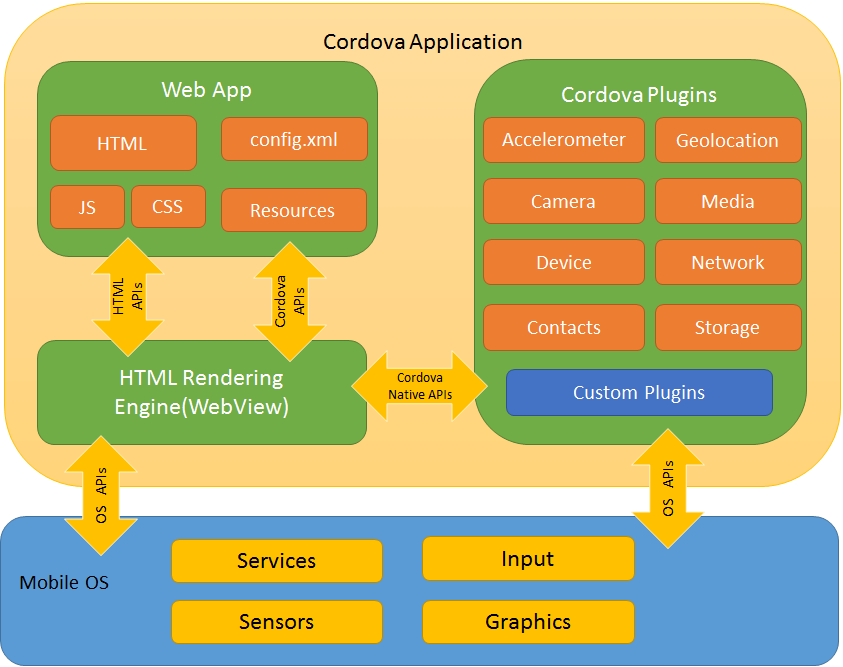
\includegraphics[width=1\textwidth]{images/apache_cordova.png}
\end{figure}

Apache Cordova applications execute within wrappers targeted to each platform.  HTML5 code is embedded inside a native WebView on the device, this interface is then used to access the device’s native resources. CSS3 and HTML5 are used for rendering the application content, while JavaScript is used to develop the application logic. HTML5 provides access to underlying hardware such as the accelerometer, camera, and GPS via the use of plugins. Plugins allow developers to add native functionality via the use of Javascript to communicate directly between the native layer and the HTML5 page. 


\subsubsection{Ionic Framework}
Ionic is a free, open-source mobile SDK for developing both native and web applications. Ionic builds on top of Apache Cordova, providing tools and services for developing hybrid applications through the use of web technologies \cite{ionidocs}. The framework is built on top of AngualJs and Apache Cordova. However, recent releases allow the developer to chose from React(Javascript Library), Angular(web framework) or Vue.js(Javascript library) as a user interface framework. Ionic utilises Cordova plugins to gain access to native hardware features such as camera, GPS, accelerometer. Ionic provides a set of front-end components and services while Cordova plugins access to native hardware of the device. Combined, Ionic and Cordova create  ‘native feeling’ applications. 

\subsubsection{Ionic CLI}
The Ionic CLI tool quickly scaffolds Ionic apps and provides a number of helpful commands to developers \cite{ionicli}. Ionic can be installed and updated via the CLI. Additionally, the CLI comes with a built-in build and debugging tools and a development server. Most of the tooling in the CLI is based on Node and is managed through npm.

\subsection{3D Modeling Tools}

\subsubsection{Blender}
Blender is a  suite of tools that support the creation of animated films, visual effects, art, 3D printed models, interactive 3D applications and video games \cite{blender}. Blender’s functionality includes 3D modelling, UV unwrapping, texturing, raster graphics editing, rigging and skinning, fluid and smoke simulation, particle simulation, soft body simulation, sculpting, animating, match moving, rendering, motion graphics, video editing and compositing. Blender’s software is open source and supported on Windows, MacOs and Linux distributions. 

\subsubsection{Wikitude Encoder}
3D content within Wikitude is managed and created using Wikitude 3D format files(.wt3). This is a compressed binary format for describing 3D models, optimized for fast loading and handling of 3D content on mobile devices. The Wikitude encoder converts 3D models into a flattened representation that can be rendered and augmented using the Wikitude SDK. The converter supports mesh-based 3D models so  that animations, textures and light sources can be applied \cite{wikiencoder}. 


The Wikitude encoder is a desktop application, supported on Windows, MacOs and Linux distributions. It currently only supports the input of .FBX for WT3 conversion. However, most 3D modelling tools support exporting to .FBX format, so files can readily be prepared for encoding. 
\begin{figure}[!ht]
\caption{Wikitude Encoder Desktop Application}
\centering
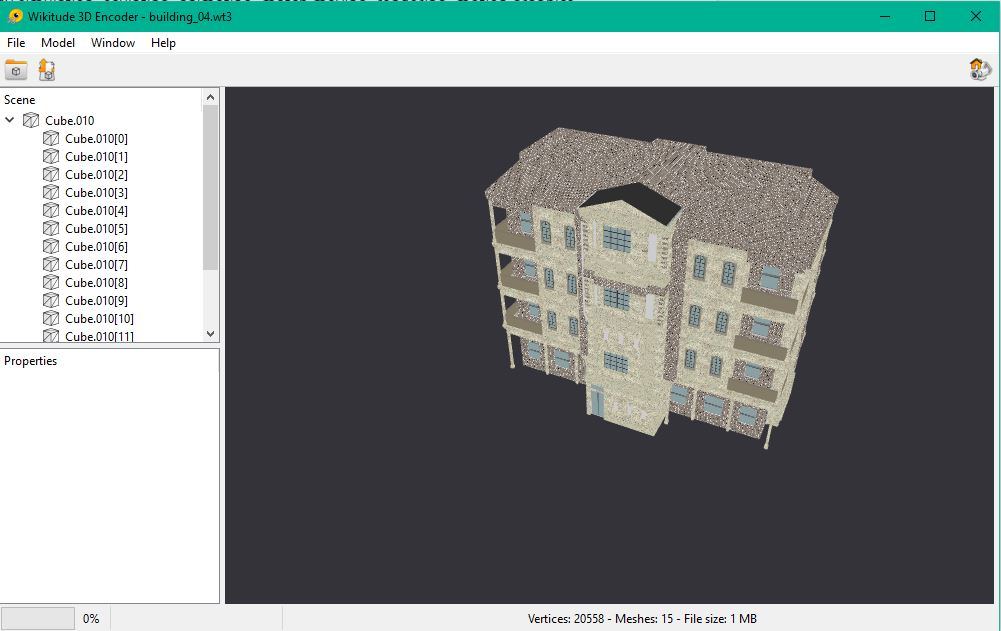
\includegraphics[width=1\textwidth]{images/wikitude_encoder.JPG}
\end{figure}


\subsection{Testing Tools}
\subsubsection{Selenium}
Selenium is a testing framework developed for web applications. Selenium is open sourced and supported on Windows, MacOs and Linux distributions. The selenium IDE is an integrated development environment (IDE) designed for creating and executing Selenium tests. It is implemented as a Firefox Add-On and as a Chrome Extension. It and allows for recording, editing, and debugging of functional tests\cite{selenium}.

\subsection{Database}

\subsubsection{Firebase}
Firebase is a platform developed by Google that provides developers with a range of tools and services to enhance mobile and web applications. Some of the features provided by Firebase include Real-time Databases, Authentication, Analytics, Hosting and Advertising\cite{firebase}. 
 \subsubsection{ Real-time Database}
The Firebase Realtime Database is a cloud-hosted NoSQL database that allows data to be stored and synced between users in real time\cite{firebase_realtime}. The database is in essence, a single JSON object. All clients share this one Real-time Database instance and automatically receive updates with the newest data.

 \subsubsection{Cloud Firestore}
Cloud Firestore is a scalable database from Firebase and  the Google Cloud Platform. Like the Firebase Realtime Database, it keeps data in sync across client apps through realtime listeners . It differs from the  real-time database in that you can upload documents and larger files for storage.

\subsection{Augmented Reality SDKs}
A selection of the top Augmented Reality SDKs were reviewed and evaluated in terms of their performance and features. The following research questions were used as criteria to examine their suitability for this project:

\begin{enumerate}
  \item What are the processes involved to implement basic AR?
\item How does it implement shared AR?

\end{enumerate}

\subsection{ARCore}

ARCore is a platform created by Google to facilitate the creation of augmented reality experiences. Using various API’s, ARCore enables mobile devices to generate a map of its environment which can then be manipulated with superimposed digital content.

ARCore makes use of the camera and sensors of the mobile device to integrate virtual content with real world surroundings. This merging of the real and virtual is achieved through three key techniques - motion tracking, environmental understanding and light estimation.



\subsubsection{Motion tracking}
 ARCore uses a process called concurrent odometry and mapping, or COM, to understand where the phone is relative to the world around it. ARCore detects visually distinct features in the captured camera image called feature points and uses these points to compute its change in location. The visual information is combined with inertial measurements from the device's IMU to estimate the pose (position and orientation) of the camera relative to the world over time. By aligning the pose of the virtual camera that renders your 3D content with the pose of the device's camera provided by ARCore, developers are able to render virtual content from the correct perspective.
 
 \subsubsection{Environmental understanding}
 ARCore creates an understanding of its environment using feature points. ARCore identifies clusters of feature points in areas containing vertical surfaces and horizontal lying objects, such as walls or tables. These surfaces are then converted into planes. ARCore identifies the boundaries of these planes, making them available to the application. This data can then be used to create an environment where virtual objects can be arranged, imparting the impression that the virtual objects are resting on the flat, real-world surface.

Using feature points to detect planes proves successful in most scenarios, however surfaces without discernible texture, for example - a white wall, may not be detected properly.

\subsubsection{Light estimation}
To create a sense of realism in the augmented reality scene, ARCore employs light estimation. Light estimation utilises the phone’s ambient light sensor in conjunction with the camera to estimate the current environment’s lighting conditions. This information is then made available to the application where colour correction and light intensity can be used to adjust the virtual objects such that they are under the same conditions as the environment.

 \subsubsection{ARCore Scenform Plugin}
 Sceneform is an Android Studio plugin for importing, viewing and building 3D assets\cite{sceneform}. Sceneform makes it straightforward to render realistic 3D scenes in AR and non-AR apps, without having to learn OpenGL. It features a high-level scene graph API and a realistic physically based renderer provided by Filament. 

\subsection{Sample Application with Sceneform \& ARCore}
For the purpose of this project, a period of time was spent investigating and developing applications using ARCore. This time was used to explore the viability of ARCore as the primary augmented reality SDK for this project.

\subsubsection{Permissions}
ARCore requires the use of the mobile device’s camera to superimpose its AR content. For this reason, the AndroidManifest.xml must be modified to indicate the application needs camera permission. 

\begin{minted}
[
baselinestretch=1.2,
fontsize=\footnotesize,
linenos
]
{xml}
<uses-permission android:name="android.permission.CAMERA" />
\end{minted}

\subsubsection{Renderables}
Sceneform uses Renderables to manage 3D content during the creation of an Augmented Reality scene. Renderables are 3D models that can be placed in any location within the scene. They consist of materials, textures and meshes. In this sample app, a renderable was created using a .obj asset file and an associated sceneform asset file.


\subsubsection{Sceneform Assets}
The Sceneform Asset Definition (*.sfa) file is a human-readable description of a sceneform asset, such a 3D model. The .sfa file contains a reference to source model paths, material definitions and textures in a source asset. The file can be automatically generated using the sceneform Android Studio plugins. It contains configurable attributes that can be modified to alter the look of an asset. The .sfa file gets built into the application's APK and is loaded at run-time to create the renderable. The syntax of the .sfa is jsonnet, an extension of JSON.
\\ \\
Sample Sceneform Asset definition: 

\begin{minted}
[
baselinestretch=1.2,
fontsize=\footnotesize,
linenos
]
{javascript}
{
   materials: [
      {
         name: "<name>",
         parameters: [
            {
               <parameterName>: <parameterDefaultValue>,
            },
         ],
         source: "path/to/source_material.sfm",
      },
   ],
   model: {
      attributes: [
         "Position",
         "TexCoord",
         "Orientation",
      ],
      file: "path/to/source_asset.ext",
      name: "<Name>",
      scale: 1.0,
      recenter: false,
      smoothing_angle: 45.0,
      flip_texture_coordinates: false,
      fix_infacing_normals: false,
   },
   samplers: [
      {
         file: "path/to/source_texture.ext",
         name: "<name>",
         params: {
            usage_type: "Color",
            mag_filter: "Linear",
            min_filter: "NearestMipmapLinear",
            wrap_s: "Repeat",
            wrap_t: "Repeat",
         },
         pipeline_name: "<pipeline_name>",
      },
   ]
}
\end{minted}
\caption{Code example provided by Sceneform documentation\cite{sfa}.}


\subsubsection{Scenefrom Scene}
The Sceneform Scene creates and maintains a scene graph. The scene graph is a hierarchical organization of a scene's content. A scene can have zero or more child nodes and each node can have zero or more child nodes.  The Scene also provides hit testing, a way to detect which node is touched by a MotionEvent or Ray.

\subsubsection{Rendering AR Content}
The ARSceneView is the class responsible for rendering and maintaining the AR content. It consists of a Scene containing all the virtual content to be rendered. 


\begin{minted}
[
baselinestretch=1.2,
fontsize=\footnotesize,
linenos
]
{java}
Node node = new Node();
node.setParent(arFragment.getArSceneView().getScene());
node.setRenderable(myRenderable);

\end{minted}



Each node contains all the information Sceneform needs to render it (including its position, orientation, and renderable object) as well as interact with it (including its collision shape and event listeners). In each frame, ARCore’s Motion tracking feature is used to compute any changes in the user’s view. Sceneform then renders the scene graph from the point of view of the Camera, guided by ARCore.

\subsubsection{Application Set up}
To use ARCore, the Sceneform plugin must be installed and imported via Android Studio. As advised in Google’s documentation, Sceneform was added to Android Studio in the following manner.

\begin{itemize}
  \item From Android Studio, navigate to Plugins settings. \\
  On Windows: File \rightarrow  Settings \rightarrow Plugins \rightarrow Browse Repositories
  \\
  \rightarrow Search -  Google Sceneform Tools
 
  \item The build.gradle file was then configured to add Google’s Maven repository. ARCore and Sceneform UX dependencies were also included.
  
  \item
    The obj model was added using the Sceneform plugin wizard, via Android Studio. The wizard automatically adds a reference to the model within the build.gradle file and generates the .sfa file. 
    
    \item In the sample app created, an XML textview element was used to render text, along with a 3D renderable. ARCore’s environment understanding identifies planes in the scene. A mesh pattern is then applied to highlight and show the user where the planes are located.

\end{itemize}

\begin{figure}[!ht]
\caption{ARCore Sceneform Application}
\centering
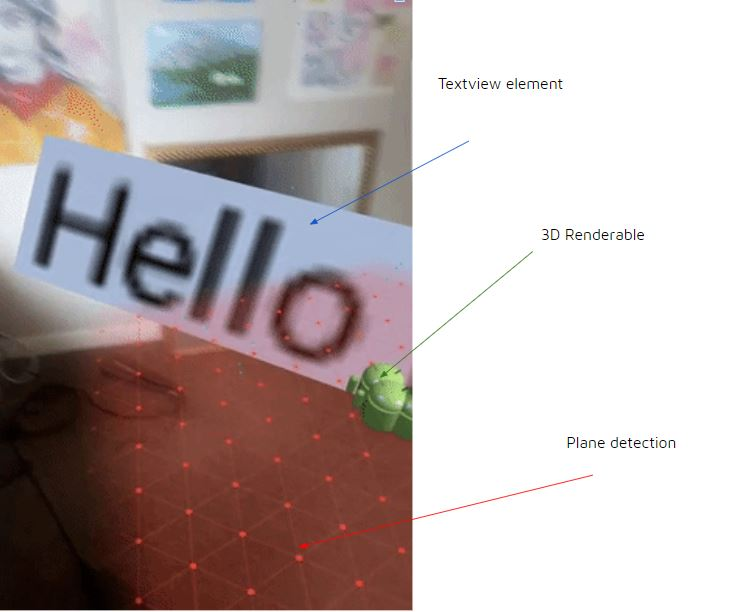
\includegraphics[width=1\textwidth]{images/sceneform_app.JPG}
\end{figure}



\subsubsection{Application Functionality}
\begin{itemize}
    \item Camera view can be moved around by the user to help find a plane.
    \begin{itemize}
        \item Triangulated mesh illustrates planes identified by plane detection algorithm.
    \end{itemize}
    
    \item On-tap listener captures user clicking area of the plane.
    
    \begin{itemize}
        \item Places an anchor and a renderable on tap location. Renderables are anchored once placed in the scene.
    \end{itemize}
    
    \item Device can be moved around and renderable with remain in place.

\end{itemize}
. 


\subsection{Shared AR with ARCore: Cloud Anchors}

Cloud anchors are Google’s approach to shared AR. Cloud anchors facilitate the creation of collaborative AR by sharing a common frame-of-reference, enabling multiple users to place virtual content in the same real-world location that can be seen on different devices in the same position and orientation relative to the environment[1]. 
\\
\\
Anchors are the fundamental element in ARCore. Anchors are estimates relating to a fixed location and orientation in the real world. Anchor poses are automatically adjusted by ARCore as its understanding of the environment improves based on the device's motion.
\\ \\
Cloud anchors are anchors that are assigned a unique ID and then uploaded to the ARCore Cloud anchor service. Once the anchor is hosted successfully the cloud anchor ID can be shared and resolved by other users. During this process, a new anchor with the original anchor's pose is assigned to the physical environment. The anchor’s pose is updated in real time on all devices accessing the cloud anchor.

The ARCore plugin for Android Studio provides support for developing applications with cloud anchors on Android devices. However, one of the key features in building a fully encompassing shared AR experience is creating an application that supports multiple platforms. For this reason, Unity in conjunction with the ARCore plugin was used to test the cloud anchor functionality. The ARCore plugin for Unity allows applications to be developed in a single codebase and then exported to both iOS and Android platforms. 

\subsubsection{Application Set Up}

\begin{itemize}
    \item A 3D Unity project was first created. In Unity’s Build Settings the target platform can be selected. For the purpose of this example, the Android platform was chosen but it should be noted iOS can also be selected for targeting Apple devices. 
    
    \item As directed in Google’s codelab demo \cite{arcore_codelab}, a basic AR scene was composed using ARCore’s First Person Camera prefab. To utilise ARCore’s environmental lighting feature, the Environmental Light prefab was also added to the Unity Scene.  Following this, a DetectedPlaneVisualizer prefab was included to illuminate the planes in the scene. 

    
    \item  With a basic application established, Cloud anchor functionality was then added. To use the ARCore Cloud Anchor API, an API key must first be obtained. Keys are available for free(limited usage) from the Google Cloud Platform. The key was added to the project via Unity’s Project Settings. The Cloud Anchor example scene provided in the ARCore package was then configured and added to the application. 
    
    
\end{itemize}

\begin{figure}[!ht]
\caption{ARCore Cloud Anchors Application}
\centering
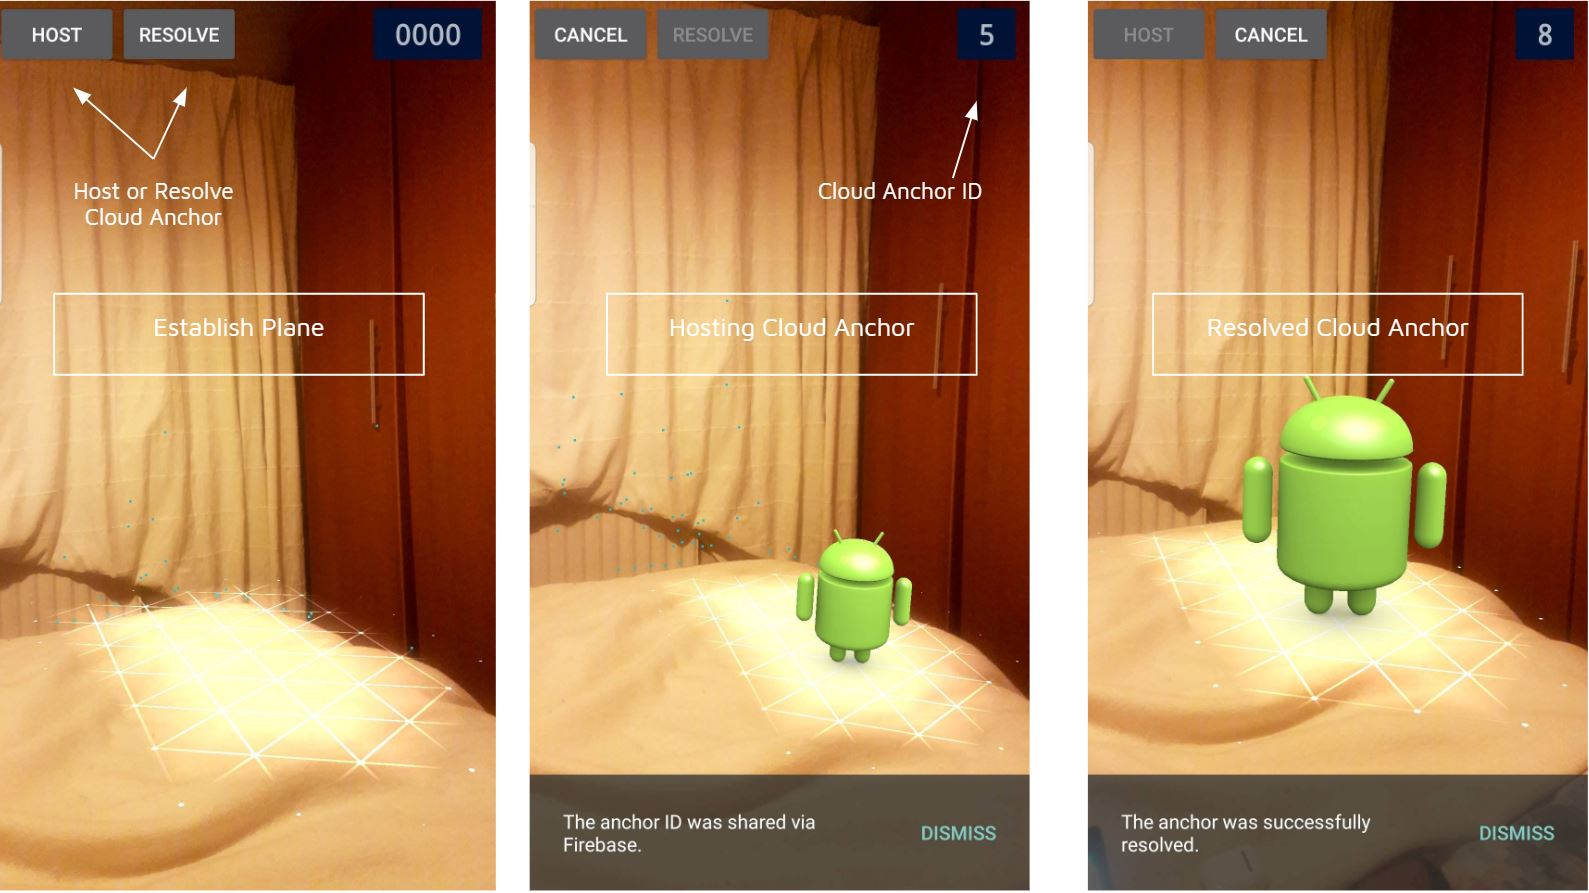
\includegraphics[width=1\textwidth]{images/cloud_anchors.JPG}
\end{figure}


\subsubsection{Application Functionality}

\begin{itemize}
    \item Camera can be moved around by the user to help find a plane. A Triangulated mesh illustrates planes identified by the plane detection algorithm.
    
    \item  On-tap listener captures user clicking an area of the plane. 
    
    \begin{itemize}
        \item Triggers the placement of an anchor and a renderable on tap location. Renderables are anchored once placed in the scene.
        \item Device can be moved around and renderable with remain in place.
    \end{itemize}
    
    \item A room number is created for the AR session(users may have multiple AR sessions).
A user wishing to join the AR Room can do so by entering a valid room number along with the user who hosted the room’s IP address. This is needed since any one user can create multiple rooms for the same physical environment.

\item The resolve button triggers a scan of the environment via the device’s camera. Distinct visual features are captured by the camera and uploaded to the cloud. The server tries to match these features with the spatial mapping of the host anchor.
If there is a successful match, the host anchor is loaded and placed in physical space. 
    
\end{itemize}

\subsubsection{ARCore Evaluation}
Creating a basic application using ARCore and Android Studio proved somewhat complex. While the initial documentation and code samples provided by Google are helpful and informative - moving away from these and trying to implement a custom application required a considerable amount of tweaking and changing small elements in various areas of code. For this reason, the learning curve associated with developing Android applications with ARCore could be considered quite high. However, this gives the developer a fine degree of control over the AR scene created, along with a range of options for customizability.

ARCore’s support for shared AR is straightforward to implement. The adoption of Unity to create cross-platform applications using the ARCore plugin was found to significantly expedite the development process. ARCore’s helper assets and configurable prefabs are clear and simple, allowing the quick assembly and implementation of a shared AR experience.  
Furthermore, the cloud anchor system proved robust when tested with multiple devices and AR sessions. 

In terms of suitability for this full stack application, ARCore and Unity lacked the key features required for this project. Unity is a game development platform, and as a result, the nature of its functionality and features are based on game development. Creating elements core to a complete mobile application, such as the user interface, navigation and database management is complex and cumbersome with Unity, as these elements are not the focus of the platform. To combat this, the insertion of a Unity ‘view’ into a framework that handles UI components such as Ionic was explored. However, this proved unsuitable as it was extremely taxing on the mobile device’s CPU, resulting in unstable and erratic behaviour within the application. 


\subsection{Wikitude}
The Wikitude SDK is a software library and framework for mobile applications used to create augmented reality experiences. The SDK supports location-based augmented reality, along with image recognition and tracking based augmented reality \cite{wikitude_docs}.


\begin{figure}[!ht]
\caption{Wikitude Architecture \cite{wikitude_docs}}
\centering
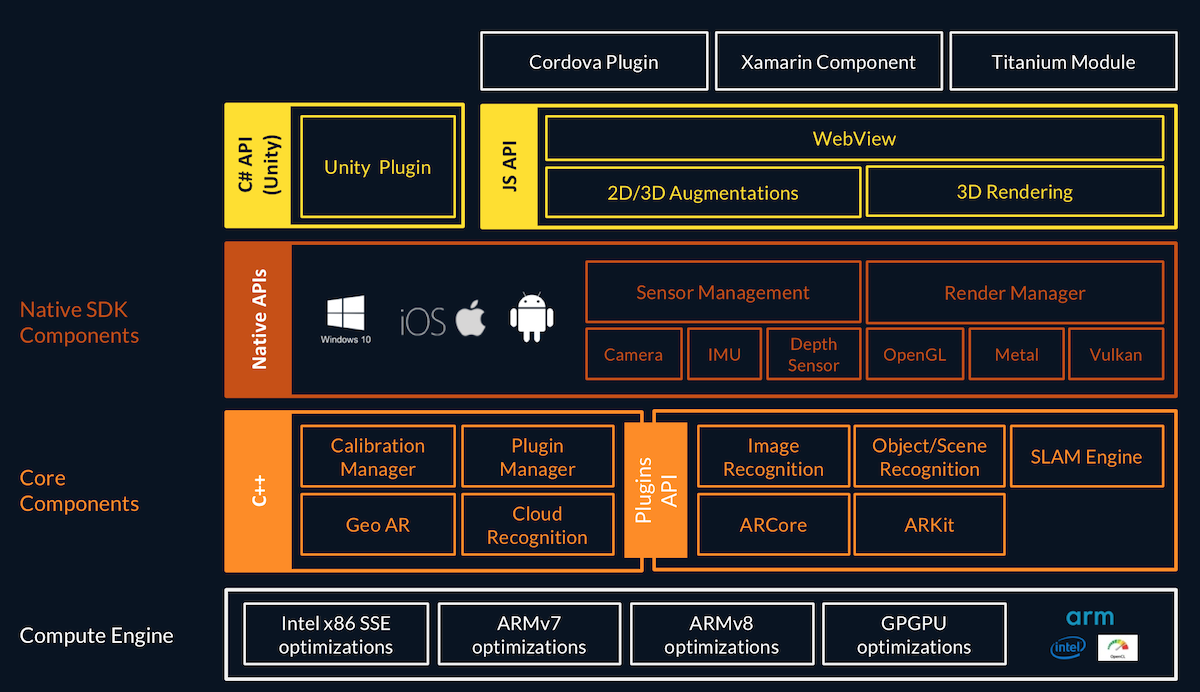
\includegraphics[width=1\textwidth]{images/wikitude_architecture.png}
\end{figure}

The image above shows the different components of the Wikitude SDK. Wikitude allows for the creation of augmented reality apps in a myriad of development environments and platforms. Platforms and extensions currently supported by Wikitude include Android, iOS,  Cordova, Titanium, Xamarin, Unity, Epson Moverio smart glasses and Vuzix

\subsubsection{ARchitect World}
The Wikitude SDK leverages web technologies to allow the creation of cross-platform augmented reality experiences. These augmented reality experiences are called ARchitect worlds. ARchitect worlds are HTML pages that can utilize the ARchitect API to generate objects in augmented reality.

The core concept is to insert an architectView to the project, (usually, a file named [projectname].html located in ./assets directory)and then notify it about lifecycle events. The architectView creates a camera surface and handles sensor events such as user tap, click or drag motions. The experiences are written in HTML and JavaScript and call methods in Wikitude's AR-namespace (e.g. AR.InstantTracking).

\subsubsection{SLAM}
SLAM (Simultaneous Localization and Mapping) is a computer vision technology that creates an understanding of the physical world through the use of feature points \cite{slam}. SLAM uses only visual inputs to perform location and mapping, meaning that the only sensor required is a camera. A feature point map is constructed and continuously updated. The agent’s location within this map is simultaneously recorded and tweaked as the understanding of environment evolves.  Wikitude provides SLAM technology via its Instant Tracking feature.

\subsubsection{Instant Tracking}
Instant Tracking is the principal algorithm that provides tracking functionality in the Wikitude SDK. The algorithm has two primary phases, the Initialization State and the Tracking State. 
\\ \\
During the initialization state, the height of the users’ device is provided in order to accurately adjust the scale of augmentations within the scene.  The tracking device height is described by the developer before run-time. The user is required to point the device so that the alignment indicator is in a stable position. Once the alignment is found to be satisfactory (the users must actively confirm), the ground plane for the AR scene is established. 

\begin{figure}[!ht]
\caption{Wikitude Instant Tracking }
\centering
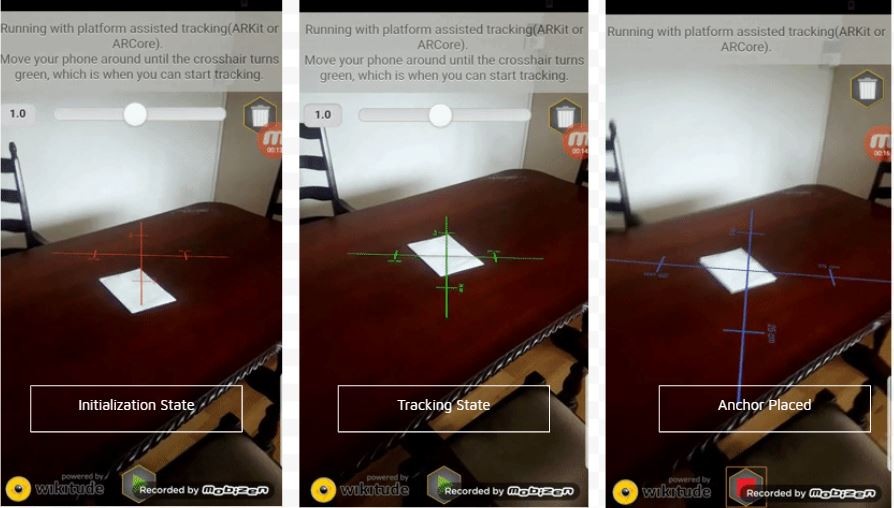
\includegraphics[width=1\textwidth]{images/wikitude_tracking.JPG}
\end{figure}

The tracking state commences once the plane has successfully been established.  In this state, the environment is being tracked continuously, which allows for augmentations to be placed within the scene.

\subsubsection{Instant Tracking Implementation}
Wikitude provides access to the instant tracking algorithm via two classes, AR.InstantTracker and AR.InstantTrackable. 

\subsubsection{Instant Tracker}
An InstantTracker represents an instance of the instant tracking algorithm. It does not require any pre-existing target information and so, can immediately start tracking. Minimally, It can be instantiated without any parameters in the following manner: 


\begin{minted}
[
baselinestretch=1.2,
fontsize=\footnotesize,
linenos
]
{javascript}

 this.tracker = new AR.InstantTracker();
\end{minted}

To ensure the most accurate tracking information, it is ordinarily instantiated with the device height. The onChangedStateFn() callback function allows the developer to invoke functionality when the tracking algorithm changes state (from initializing to tracking).

\begin{minted}
[
baselinestretch=1.2,
fontsize=\footnotesize,
linenos
]
{javascript}

this.tracker = new AR.InstantTracker({
    onChangedState:  function onChangedStateFn(state) {
        // react to a change in tracking state here
    },
    // device height needs to be as accurate as possible to have an accurate scale
    // returned by the Wikitude SDK
    deviceHeight: 1.0,

 // The initial orientation at which the instant tracking plane should be displayed in degrees.
 // Default value is AR.CONST.INITIAL_INSTANT_TRACKING_PLANE_ORIENTATION.HORIZONTAL (0°).
    trackingPlaneOrientation: 45.0
});

\end{minted}
\caption{\cite{instant_tracking}}

\subsubsection{Instant Trackable}
The InstantTrackable Class describes a virtual object attached to an InstantTracker. Drawable augmentations can be bound to an instance of InstantTrackable, allowing them to receive relevant transformations during the tracking state. An InstantTrackable may also take the form of a tracking plane. Triggers can be connected with InstantTrackers to invoke events and functions to react to changes in the tracking state.  \\ \\
To create an instance of the InstantTrackable Class, an InstantTracker object must be passed as a parameter to its constructor. 

\begin{minted}
[
baselinestretch=1.2,
fontsize=\footnotesize,
linenos
]
{javascript}

this.instantTrackable = new AR.InstantTrackable(this.tracker, {
    drawables: {
        cam: aDrawable,
        initialization: anotherDrawable
    },
    onTrackingStarted: function onTrackingStartedFn() {
        // do something when tracking is started (recognized)
    },
    onTrackingStopped: function onTrackingStoppedFn() {
        // do something when tracking is stopped (lost)
    }
});


\end{minted}
\caption{\cite{instant_tracking}}

\subsubsection{SMART - Seamless AR Tracking}
SMART is an API which integrates ARKit, ARCore and Wikitude's SLAM to provide multi-platform sugmented reality tracking. The goal of SMART is to ensure the most accurate AR tracking for the device in use. The SMART API checks the platform of the device. If it is identified as an Android device, it then checks whether it is supported by ARCore, if so - it loads ARCore’s methods for improved tracking. Similarily, if the device runs iOS, ARKit’s tracking algorithms are used. If the device is not supported by either ARcore or ARKit - Wikitude's SLAM/basic Instant tracking algorithm is used. 

SMART is enabled by default but can be disabled by setting a parameter when creating an AR.InstantTracker with the smartEnabled option. The behaviour cannot be changed during runtime.

\begin{minted}
[
baselinestretch=1.2,
fontsize=\footnotesize,
linenos
]
{javascript}

new AR.InstantTracker({
    smartEnabled: false
});

\end{minted}
\caption{\cite{instant_tracking}}


SMART provides improved tracking capabilities at the expense of control. Therefore, some of Wikitude’s features are not available when platform tracking capabilities are used by enabling SMART. The following figure illustrates the functionality available with SMART tracking activated. 

\begin{figure}[!ht]
\caption{SMART Compatibility}
\centering
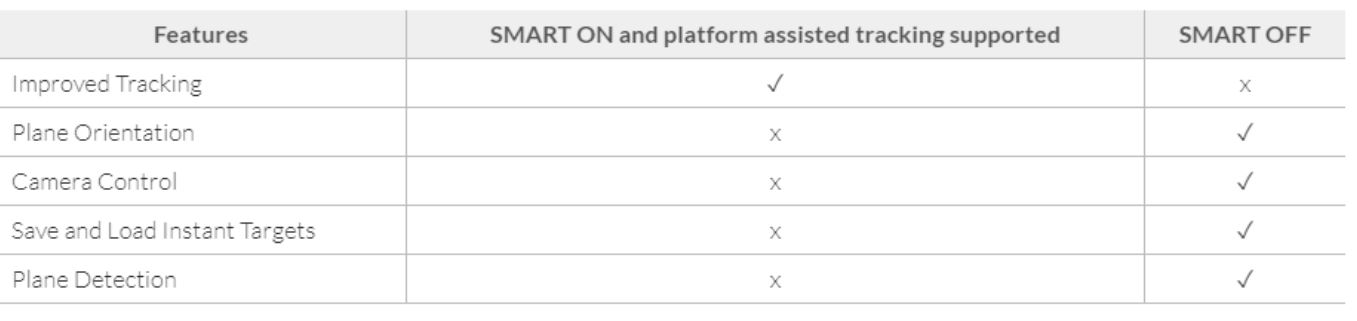
\includegraphics[width=1\textwidth]{images/smart.JPG}
\end{figure}

\subsubsection{Object and Scene Recognition}
Object Recognition and Tracking let you detect objects and entire scenes that are pre-defined by the developer. The scene and object recognition feature is based on Wikitude's SLAM engine, which is used throughout the SDK for environment tracking. The object recognition feature tries to find and match a pre-created reference in the live camera image. This pre-created reference is called  an Object Target. Object Targets can be created using videos or images as source material. The source material is converted into a Wikitude Object Target Collection, which is stored as .wto file \cite{wikitude_docs}. Wikitude’s studio Manager is a free web tool that helps manage and create object targets. 

\subsection{Augmenting 3D Content}
\subsubsection{AR.Model}
The AR.Model class represents a drawable AR object as a 3D model. The Model type consists of a link to a .WT3 file that has been created using the Wikitude Encoder. During a model’s instantiation, setup parameters can be provided to allow for customization of its properties, for example, the model’s scale and rotation. 
\\ \\
The following example illustrates the initialization of a Wikitude Model
\begin{minted}
[
baselinestretch=1.2,
fontsize=\footnotesize,
linenos
]
{javascript}

//create a new Model and pass some setup parameters
var model = new AR.Model("models/my3dModel.wt3", {
  // scales it to half of the original size
  scale: {
    x: 0.5,
    y: 0.5,
    z: 0.5
  },
  // rotates it 90 degrees around the z-axis and 180 degrees around the x-axis
  rotate: {
    x: 180.0,
    y: 0.0,
    z: 90.0
  },
  // moves the 0bject 5 SDUs along the x- and the y-axis
  translate: {
    x: 5,
    y: 5,
    z: 0
  },
  onClick : function() {
    //something happens
  }
}
\end{minted}
\caption{\cite{instant_tracking}}


\subsection{Shared AR with Wikitude: Persistent Targets}
The Wikitude SDK  does not officially support functionality for Shared AR. However, as the SDK uses JSON objects to build AR experiences, the Persistent Instant Targets feature has emerged as a manner of exploiting this to dynamically save and load AR experiences. By essentially saving and loading a stringified JSON object representing the AR scene, it is possible to create shared AR that may be persistently accessed by multiple users across devices and operating systems. 


\subsubsection{Save Instant Target}
To save an AR experience, an active InstantTracker in the tracking state must be present in the ARchitect world. The Save Instant Targets functionality calls on the AR.platform.sendJSONObject method to send the current AR scene as a JSON object to the platform.  
\begin{minted}
[
baselinestretch=1.2,
fontsize=\footnotesize,
linenos
]
{javascript}

 if (this.tracker.state === AR.InstantTrackerState.TRACKING) {
        AR.platform.sendJSONObject({
            action: "save_current_instant_target",
            augmentations: JSON.stringify(augmentations)
        });
    }
    
\end{minted}
\caption{\cite{instant_tracking}}
The AR scene’s current models, scaling, rotations and positioning are bundled into an the augmentations object and sent from the ARchitect world to the platform.

\subsubsection{Load Instant Target}
In order to load an instant target, a path to a valid JSON object representing an AR scene’s augmentations must be provided. Similar to the process of saving an AR scene, to load one, AR.platform.sendJSONObject and architectView.callJavaScript are used. 

\begin{minted}
[
baselinestretch=1.2,
fontsize=\footnotesize,
linenos
]
{javascript}
// Inform the platform code to load a AR scene
loadExistingInstantTarget: function () {
    AR.platform.sendJSONObject({
	// triggers this method on the platform side code
        action: "load_existing_instant_target"
    });
}
\end{minted}
\caption{\cite{instant_tracking}}

The platform code receives the call to load an AR scene and proceeds to do so in a manner custom to the application. For example, the augmentation may be loaded from a local file on the device or a remote database. 

\subsubsection{Wikitude Evaluation}
Creating applications utilising the Wikitude SDK has numerous benefits. As the SDK is based on web technologies, it leverages significant flexibility. This is evident in the diverse platforms it currently supports. Furthermore, Wikitude’s SMART API provides support for 92.6\% of iOS devices and roughly 35\% of Android devices available on the market\cite{instant_tracking}. In contrast, ARCore currently only supports 28.2 percent of Android devices currently available \cite{android_stat}.

Documentation and support for shared AR with Wikitude is lacking in comparison to that of ARCore. Nevertheless, the underlying technology remains open to develop and build upon. Although this is more work for the developer, it yields greater control and autonomy over its implementation. 

While ARCore may be considered more robust as its underlying codebase is developed in C\#, Wikitude’s use of Javascript and JSON promote rapid development when utilising the SDK. Additionally, Wikitude can be easily integrated with a wide range of technologies in the development of a full-stack application. For example, the SDK can be used in conjunction with platforms such as Ionic and Apache Cordova to create cross-platform applications. 

Given its use of web-based technologies and wide range of supported devices, Wikitude's SDK was deemed most suited to this projects goal of creating a full stack, cross platform application.
